
\chapter{関連研究}
\label{chapter:related_work}
本章では, これまでに報告されている複数経路利用によるフロー完結時間短縮化技術について簡潔に述べ, その優位性や問題点を示す.
大量のネットワーク機器により構成されており, 短時間で大量のデータの処理を行うデータセンターネットワーク環境において,
リクエストに対するレスポンスの高速化によるユーザエクスペリエンスのさらなる向上が求められており, 低レイテンシなネットワークが必要とされている. 
本章では, これまでに報告されているデータセンターにおける低レイテンシなネットワークに関する研究について述べる. 
既存の研究では, キュー長の縮小, 再送処理の高速化, ショートフローの優先付け, 複数経路の利用の4つの技術を用いることで実現しており,
4つの分類ごとにその特徴や課題について考察する. 
そして, 本研究の位置付けを示す. 



\begin{table}[t]
\begin{center}
{\footnotesize
\begin{tabular}{c|c|c|c|c|c|c|c}
\hline
\multicolumn{2}{c|}{\multirow{2}{*}{Categories}} &
\multirow{2}{*}{Proposals} &
\multicolumn{2}{c|}{Objectives} & 
\multicolumn{3}{c}{Modifications to} \\\cline{4-8}
\multicolumn{2}{c|}{ } &  & FCT & deadline & TCP & Switches & applications \\
\hline
\multicolumn{2}{c|}{\multirow{2}{*}{Redcing queue length}} &
DCTCP & mean & $\times$ & $\surd$ & $\times$ & $\times$ \\ \cline{3-8}
\multicolumn{2}{c|}{ } & HULL & mean & $\times$ & $\surd$ & $\surd$ & $\times$
\\ \hline

\multirow{6}{*}{\parbox{8zw}{Prioritizing flows basd on}} &
\multirow{4}{*}{\parbox{6zw}{Flow deadlines}} & ${\rm D^3}$ & none &
 $\surd$ & $\surd$ & $\surd$ & $\times$ \\ \cline{3-8}
 
 & & PDQ & none &
 $\surd$ & $\surd$ & $\surd$ & $\times$ \\ \cline{3-8}
 
 & &${\rm D^2TCP}$ & tail &
 $\surd$ & $\surd$ & $\times$ & $\times$ \\ \cline{3-8}
 
 & & MCP & tail &
 $\surd$ & $\surd$ & $\times$ & $\times$ \\ \cline{2-8}

 &\multirow{2}{*}{\parbox{6zw}{Application assignment}} & pFablic &
 \parbox{3zw}{\strut{}mean \& tail\strut} & $\surd$ & $\surd$ &  $\surd$ &
 $\surd$
 \\
 \cline{3-8}
 
 & & \multirow{2}{*}{Detail} & \multirow{2}{*}{tail} &
\multirow{2}{*}{$\surd$} & \multirow{2}{*}{$\surd$} &
\multirow{2}{*}{$\surd$} & \multirow{2}{*}{$\surd$} \\ \cline{1-2}

\multicolumn{2}{c|}{\multirow{2}{*}{Exploiting multipath}} & & & & & \\
\cline{3-8}

\multicolumn{2}{c|}{ } & RepFlow & \parbox{3zw}{\strut{}mean \& tail\strut} &
$\times$ & $\times$ & $\times$ & $\surd$ \\ \hline

\multicolumn{2}{c|}{\multirow{3}{*}{Accelerating retransmissions}} & DIBS & tail
& $\times$ & $\surd$ & $\surd$ & $\times$ \\ \cline{3-8}

\multicolumn{2}{c|}{ } & FastLane & tail
& $\times$ & $\surd$ & $\surd$ & $\times$ \\ \cline{3-8}

\multicolumn{2}{c|}{ } & CP & tail
& $\times$ & $\surd$ & $\surd$ & $\times$ \\ \hline

\end{tabular} 
}
\caption{An overview of low latency datacenter networking proposals}
\label{table:proposal_list}
\end{center}
\end{table}

\section{キュー長の縮小}
レイテンシの大きいデータセンターネットワークの主な原因はキューイング遅延である\cite{dctcp}. 
報告された解析結果\cite{dctcp}によると, ネットワーク全体のトラフィック量が比較的小さく, 大きな輻輳が発生していない環境においても,
ショートフローのFCTの大部分がキューイング遅延に依存する. 
キューイング遅延を減らし, FCTを改善するための一つの手法として, キュー長の縮小がある. 

スイッチのキュー長を減らし, バッファの占有を抑えることにより, 遅延を改善するというアプローチは最も直接的な手法である. 
高速にパケット処理のできない汎用的なスイッチではバースト性のあるトラフィックに対して, バッファを多く用意することで対応している. 
データセンターネットワークでは基本的に帯域遅延積が小さく, バッファが大きいと通信性能に影響が出る. 
既存のTCPの輻輳制御では, ロングフローがバッファを使い切るまで通信しようとし, それにより大きなキューイング遅延が生まれ,
ショートフローの通信性能に影響が出る. 
そのため, キューイング遅延を抑えるために, スイッチのバッファを小さくし,
新しい帯域制御手法や輻輳検出のための仕組みがエンドノードとスイッチに対して必要となる. 

DCTCP\cite{dctcp}とHULL\cite{hull}はスイッチバッファの占有率を持続的に低く保ち, 遅延を抑える為に提案された手法である. 

\subsection{DCTCP}
DCTCP(Data Center TCP)\cite{dctcp}はデータセンターネットワーク内の遅延問題の解決を目指した初めての取り組みである. 
Alizadehら\cite{dctcp}は実際に稼働しているデータセンターのトラフィックを観測, 1ヶ月分のトラフィックデータの解析を行い,
データセンターネットワークが生成するトラフィックの特徴を考察した. 
その結果, データセンターのトラフィックの大部分がレイテンシ指向なショートフローであることを示し,
ロングフローによってバッファが占められた中継されるスイッチの影響でショートフローが大きく遅延することを示した. 
これらの観測結果が動機となり, 著者たちはスループット性能を大きく損なうことなく,
バッファの占有を抑える為の輻輳手法としてDCTCPという新しいトランスポートプロトコルを提案した. 

DCTCPは汎用的なスイッチにも広く実装されているExplicit Congestion
Notification(ECN)による輻輳通知の機能を用いている.
バッファ占有のしきい値をあらかじめ設定しておき, それを超えると,
スイッチがパケットのTCPヘッダーのECNエコーフラグを用いてエンドノードに明示的に通知する.
この情報を用いてサーバはTCP遅延ACKにECNエコーフラグを加えクライアントホストに知らせる. 
そしてクライアントでは, ECNマークされたパケットの割合によって, スイッチバッファの状態を推定し, ウィンドサイズを抑える. 
その結果, キュー溢れが起こる前に輻輳を回避することができ, バッファ占有を抑えることができる. 
DCTCPは既存のTCP実装に対して, 30行の変更を加えるだけで利用することができ, 今のインフラに対して容易に展開することができる. 
DCTCPはテストベッド環境での評価において, FCTを大きく改善することができ, 特にテール部分について,
99パーセンタイルFCTをTCPの40\%以上短縮化を達成した. 


\begin{figure}[t]
    \begin{center}
    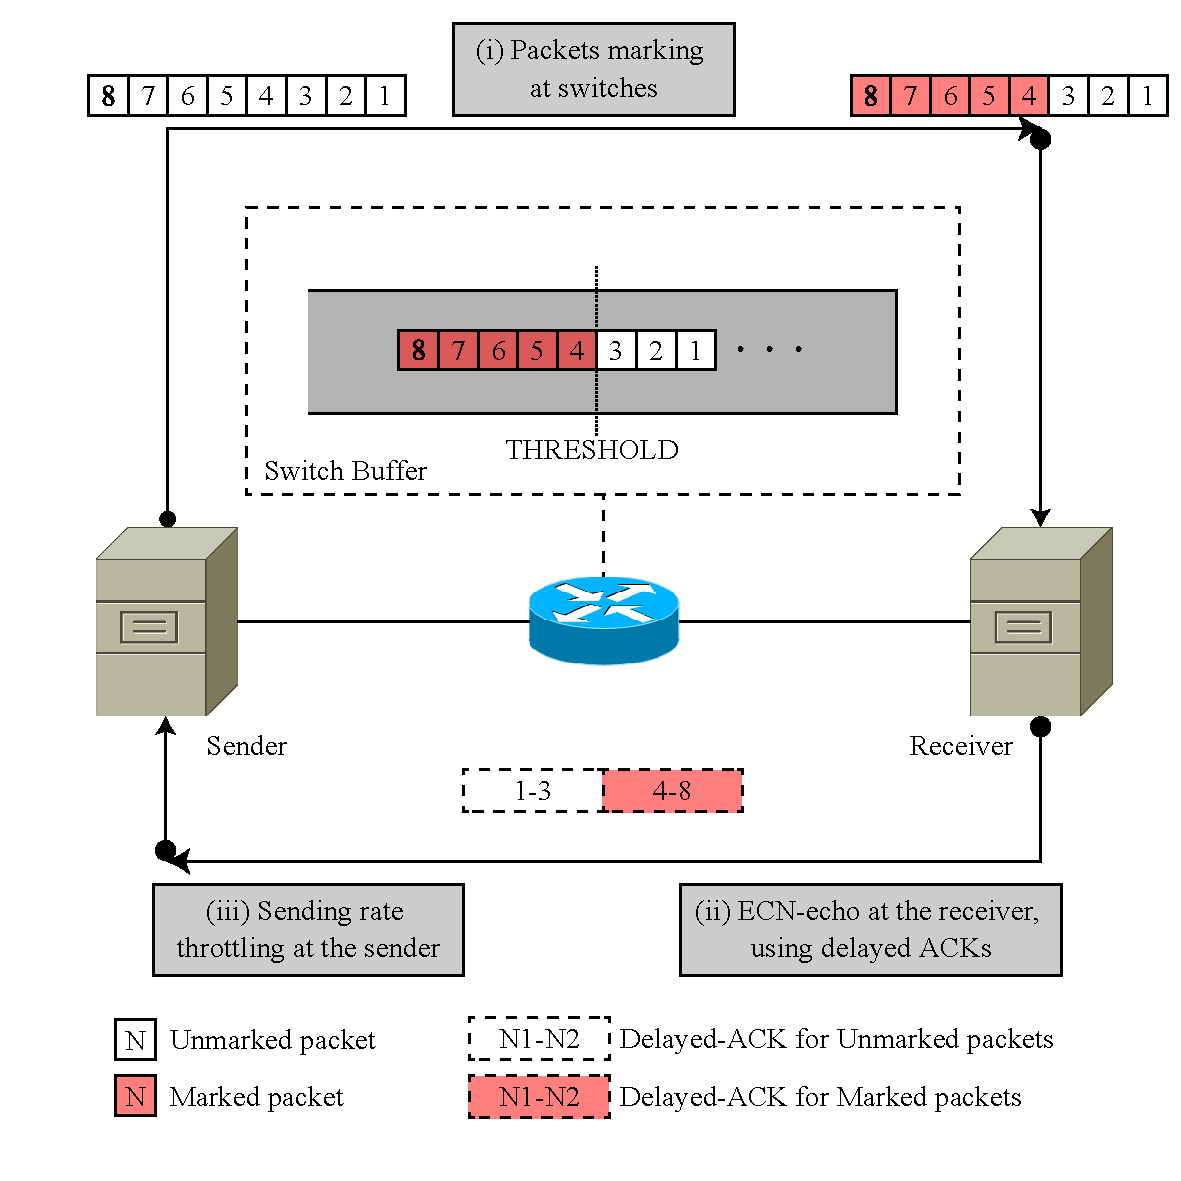
\includegraphics[autoebb, width=300pt]{./img/DCTCP.pdf}
    \caption{The control loop in DCTCP}
    %\ecaption{The control loop in DCTCP}
    \label{fig:dctcp_control}
    \end{center}
\end{figure}

\subsection{HULL}
HULL(High-bandwidth Ultra-Low Latency)\cite{hull}はDCTCP実装をベースに追加にした手法であり,
さらなるキュー長の縮小のためのすべてのポートのキュー状態の推定を目的としている. 
HULLは直接的にキュー長の様子を通知するDCTCPとは異なり, 通信利用帯域によるリンク利用率を基にした輻輳通知手法である. 

HULLではリンク利用率を用いたファントムキューという仮想キューを利用している. 
これは, バッファ処理自身のオーバーヘッド影響を考慮せず,
実際の物理リンクよりも低い通信レートでの仮想リンクにおけるキューイングの様子をエミュレートすることによって算出される. 
ファントムキューがしきい値を上回った場合, DCTCPと同じECNを用いた通知機構を用いて, ウィンドウサイズの調整を行いキュー長を抑える. 
ファントムキューは物理リンクよりも低いレートにおいてシミュレートされているため, よりレートの高い実際の環境におけるバッファではより小さく保つことができ,
キューイング遅延の影響がより小さくなる. 
著者は平均値, 99パーセンタイル値のFCT共にDCTCPの10倍以上, TCPの40倍以上改善することができたことを示した. 
しかしFCTの改善のトレードオフとして約10\%の利用帯域の減少も生じていることも示した. 

\section{再送の高速化}
データセンターネットワークの遅延を抑える為の手法として, パケットロスによる遅延に対して改善を行う手法がある. 
通常TCPでは, パケットロスが起こった場合, それを検知するためのタイムアウト時間(RTO)後に再送制御を行う. 
一般にRTOはエンドノード間のラウンドトリップ時間(RTT)よりも非常に大きな値を設定するため, RTOによって不必要な時間分だけ待たなければならない. 
これまでに提案された手法では, RTOを小さくする, あるいはRTOによる再送制御を無視し,
明示的にエンドノードに対してパケットロスが起こったことを通知することで, 再送遅延の短縮化を実現している. 

ショートフローとロングフローの両方が共存している場合, パケットロス, 再送制御が起こることは避けられれない. 
パケットロス自体は頻繁に起こるわけではなく, その割合も小さいため, 再送制御による遅延を改善することはテール部分の遅延の改善に対して大きく貢献する. 
TCPでは, 基本的にはショートフローのFCTはRTOよりも短いため, パケットロスが起きた場合の影響は非常に大きく,  
例えばアプリケーション性能に依存するショートフローにとって, そのFCTがデッドラインを満たすためにはRTOは大きすぎる. 
またTCPの輻輳制御では, パケットロスが起こった際に, ウィンドウサイズが減少され, フローを完結するためにより多くのラウンドトリップが必要となる. 

先行研究では, この問題を解決するために, 二つの観点からアプローチしている. 
DIBS\cite{dibs}ではパケットロスが起こった際, その混雑しているポートとは異なる他のポートをランダムに選択,
パケットをリダイレクトし再送制御を行う. 
また, FastLane\cite{fastlane}, CP(cutting
Payload)\cite{cp}では高速に明示的な通知をエンドノードにおこうことで, 再送制御を高速化する. 

\subsection{DIBS}
Detour-Induced Buffer Sharing\cite{dibs}では, アイドル状態のネットワーク資源を利用し,
ホットスポットでのバーストトラフィックを緩和させる. 
スイッチがパケットロスをしなければならない時, 本来転送しなければならないポートとは異なる他のポートをランダムに選択し, パケットを転送する. 
これにより3つの成果を生み出すことができる. 
\begin{enumerate}
\item 他のパスに転送されることでより多くのホップ数を必要とする可能性があるが, 輻輳が起こっているホットスポットを避けることができる. 
\item 転送したパケットがループバックしてきた際に,
本来転送するべきポートのバッファが占有されていないパケットロスが起こらない状態であればそちらに転送する.
\item そのパケットのTTLに達するまでに, アイドル状態のパスを見つけられなかった際には, パケットは破棄される. 
\end{enumerate}
複数の等価コストのパスをもつデータセンターネットワークの性質上, 迂回経路によって大部分のパケットロスを抑えることができる. 
また, アイドル状態のパスを見つけられない可能性はデータセンターでは低いが, その際にはタイムアウトや再送制御が行われる. 

\subsection{FastLane, CP}
FastLane\cite{fastlane}とCP\cite{cp}は再送制御の高速化のための明示的なパケットロスの通知を生成する. 
それにより, 再送制御を起動させるまでのオーバヘッドをRTO時間から1回分のラウンドトリップへと減少させる. 

FastLane\cite{fastlane}は, パケットロスを引き起こしたスイッチで検出し, 直ちにエンドノードへ通知を行う. 
CPUのオーバーヘッドを抑えるために, ロスを引き起こしたパケットのIPアドレスをスワップし, エンドノードへ通知する. 
これにより, エンドノードはどのフローでパケットロスが発生したかを素早く知ることができる. 
また, 通知するためのトラフィックに対し, 通信帯域の制限(bandwidth cap)をすることで,
ネットワーク全体の帯域オーバーヘッドを抑えることができる. 
一方, CP\cite{cp}は通知のために新しいパケットヘッダーを用いる. 
パケットロスが起こった時に, ペイロードの大きいパケットについてはペイロード部分を取り除く. 
通知を受けたノードは, ヘッダーを見てペイロードが除去されていることを認識し, 
SACKのようなピンポイントでのACKによって再送制御を呼び出す. 
FastLaneもCPもどのトランスポートプロトコルと互換性を持つ手法である. 

\section{ショートフローへの優先付け}
ショートフローのFCTを改善するための手法として, 優先制御がある. 
どのパケットも同じ扱いをするTCPとは異なり, ショートフローに対しては優先度を高く設定し,
他のキューイングされているパケットよりも前に処理されるような優先制御が行われ, それによりショートフローのFCTが大きく改善される. 
フローの優先付けには二つの方法がある. 
一つは, アプリケーションによって明示的に優先度を定められ, 優先度を割り当てられる手法\cite{p_fab, detail}. 
もう一方は, 今日のデータセンターの扱うアプリケーションが暗黙的に定めるデッドライン情報を用いて優先度を割り当てる手法である. 
いくつかのアプリケーションでは各フローに対しておよそ200ms$\sim$300msのデッドラインを満たす要求があり, 優先制御によりそれを実現し, 
また, そうしたデッドラインが明示的に定められないものについては, レスポンス時間を保証するために用いられる\cite{mcp, pdq, d2tcp, d3}.
そのため, ネットワーク内のスケジューリングによるフローの優先付けは既存のトランスポート層,
データリンク層のプロトコルを改良することで効果的な手法が実現される. 

一般的に, インターネットにおける通信の公平性では, ロングフローであるかショートフローであるかに依らず, どのパケットも公平に扱おうとし,
多くの手法がそれに従っている. 
しかし, データセンターネットワークでは, ロングフローによるショートフロー通信性能の劣化を引き起こす中で,
こうした考えは, 不公平であるという議論もある\cite{mcp, pdq, d2tcp, d3}.
そうした不公平性の問題を解決するために優先制御手法が提案されているが, 大きく2種類の情報を使う手法に分類することができる. 
一つは, フローのFCTのデッドラインによって優先度を決める手法. 
他方はアプリケーションによって明示的な優先度を設定される手法がある. 

\subsection{デッドラインベースの優先付け}
\subsubsection{${\rm D^3}$}
${\rm D^3}$ (Deadline Driven Delivery)\cite{d3}はデッドラインベースの優先制御手法である. 
${\rm D^3}$では, フローのデッドラインを満たすために必要な帯域を割り当てることによってネットワークリソースの最適な配分ができるという考えに基づいている. 

Wilsonら\cite{d3}は, サーバとクライアントでインタラクティブな通信を必要とする多くのアプリケーションは,
そのアプリケーションフローを生成する処理ノードによってデッドラインが定められていると述べており, このデッドライン情報を用いることで,
$ {\rm D^3}$はデッドラインまでに通信を完了できる最小のレートを算出し, パケットのヘッダー情報として追加する. 
それにより, フローは中継するすべてのスイッチに対して必要な帯域を要求することができる. 
スイッチはACKパケットによってそのリクエストに対する予約帯域をエンドノードに通知する
そしてクライアントノードはその通知に従って送信レートを調整する. 

${\rm D^3}$が適用されるスイッチでは, 計算, メモリー容量を抑えるため, スイッチによる帯域割り当ては,
FCFS(first-come-first-serve)に基づいて実行される.
そのため, すべてのフローに対して要求を満たすための帯域が不十分な状況であれば, 先着順で初めのいくつかのフローしか満たせない可能性もある. 

\subsubsection{PDQ}
${\rm D^3}$のFCFSスケジューリングは十分なパフォーマンスを引き出せない場合がある. 
十分にパフォーマンスが引き出せない状況について, Fig\ref{fig:fair_share}に示す. 
こうした公平性の考えがPDQ(Preemptive Distributed Quick)フロースケジューリングの設計指針となっている. 
PDQは${\rm D^3}$のスケジューリングに対して横取りスケジューリングをすることを許可し,
デッドラインを素早く満たせるフローについては積極的に帯域を割り当てるような制御を行う. 

PDQでは, デッドラインが短いフローから, サイズが短いフローから, の二つの規律に従ってスケジューリングを行っている. 
このスケジューリングを実現するために, 分散スケジューリングレイヤーによって, 他のスイッチと連携を取り, 安定的な帯域割り当てを実現する. 
PDQによるスケージュリングはFIFO droptail キューを用いて近似的に実現している. 
シミュレーションによる実験では, 現実世界でのトラフィックでの検証を行い, ${\rm D^3}$に対して, 平均FCTを30\%以上改善することができたと報告している. 

\begin{figure}[t]
    \begin{center}
    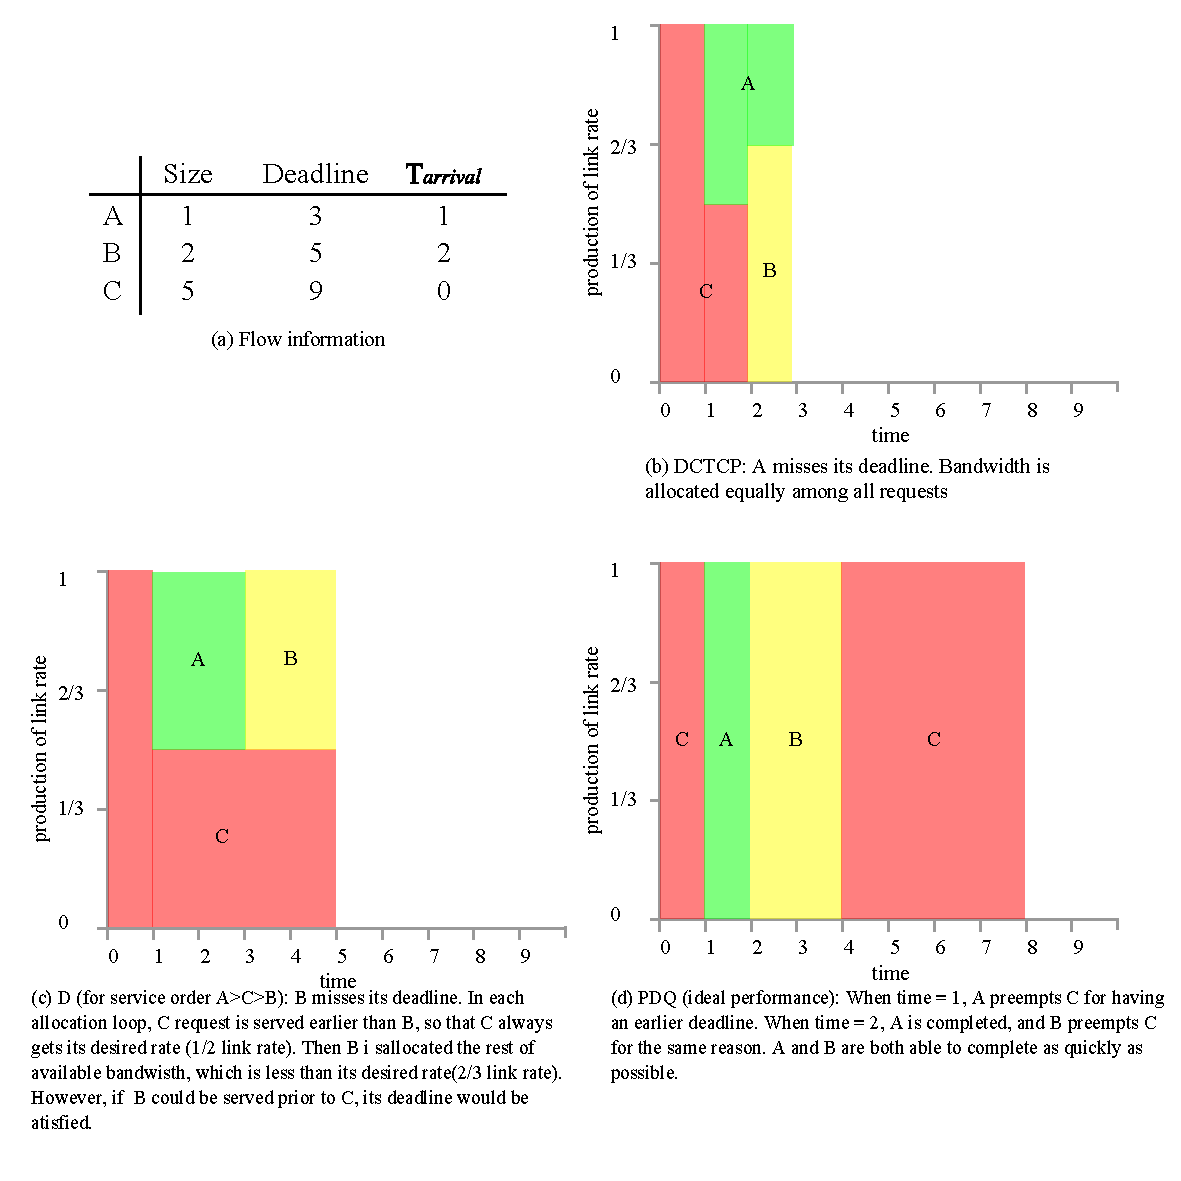
\includegraphics[autoebb, width=300pt]{./img/fair_share.pdf}
    \caption{Fair-share(e.g. DCTCP)and ${\rm D^3}$ are sub-optimal in meeting
    deadline}
    %\ecaption{The control loop in DCTCP}
    \label{fig:fair_share}
    \end{center}
\end{figure}

\subsubsection{${\rm D^{2}TCP}$, MCP}
$ {\rm D^{2}TCP}$\cite{d2tcp}, MCP\cite{mcp}では, フローのTCP ウィンドウサイズを調整することで,
デッドラインを満たす制御を行う.
いずれの手法も, ECNによって輻輳状態を推定するDCTCP\cite{dctcp}を基にした手法で,
DCTCPの手法にフローのデッドライン情報を考慮に入れた, 優先制御を実現している. 

${\rm D^{2}TCP}$はガンマ補正関数を用いてデッドラインを満たすTCPウィンドウサイズに調整する. 
具体的には, デッドラインに近いフローほど, より多くのウィンドウサイズが割り当てられるような制御がされる. 
MCP\cite{mcp}はさらにもう一歩先に進んだ手法となっており, 通信が開始した直後にデッドラインを満たすようなウィンドウサイズの調整が行われる. 
具体的には, ECNベースの輻輳制御が行われ, 長期的なパケットごとの平均遅延時間を最小にする最適化問題としてアルゴリズムが実装されている. 
Chenら\cite{mcp}は最適なウィンドウサイズの割り当てを凸計画問題として解き, 数値評価によって提案した近似アルゴリズムの有用性を示している. 


\subsection{アプリケーションベースの優先付け}
\label{subsec:ap_priority}

\subsubsection{DeTail}
Detail\cite{detail}はテールFCTの改善を目的としたクロスレイヤーフレームワークである. 
Zatsらはロングテールなレイテンシを持つFCTとなる二つの主な原因を示し, それらを低減する二つの手法を提案した. 
原因の一つは, それぞれのフローの中に優先度がないことである. 
一時的な輻輳状態の際, ロングフローの継続的な通信のためショートフローが十分なデータ量が通信できなくなり, 大きく遅延するフローが発生する. 
DeTailでは, 近年標準化されたPFC(Priority Flow Control)によるQoS制御によって, データリンク層においてこの問題を解決する. 
PFCは近年のL2スイッチには実装されており,
輻輳時に優先度の低いフローについて一時的に通信を止めることによる優先制御をスイッチからエンドノードに対して通知することで実現可能である. 

二つ目の原因は, ネットワークレイヤーにおける不均一なロードバランシングである. 
現在実装されている, ハッシュベースのロードバランス手法では, 輻輳が発生していない経路が存在しているにもかかわらず,
ロングフローとショートフローが同一の経路を選択する可能性がある. 
DeTailでは, 各経路の通信状況に適応させるマルチパスロードバランス手法($\S$\ref{subsec:u-multipath})によって,
この問題を解決している.

\subsubsection{pFabric}
多くの手法が様々な仕組みを組み合わせた複雑なシステムによって遅延の改善を目指してきたが, 提案したpFabric\cite{p_fab}では,
最小限のシステムによって問題の解決を目指している. 
pFabricの設計指針は, 優先制御による利得を最大限に引き出すことである. 
Alizadehらは, フローによって通信レートを差別化する手法は広く提案されているが, それらは効果的でなく, 実装も難しく,
そうした送り手側の通信レートの制御に代わり, スイッチにおけるショートフローの優先度付けのみで十分有効であると述べている.

pFabricでは, デッドラインが短いフローや, ユーザエクスペリエンスに大きく関わるフローについてはヘッダーの優先値を設定しておき,
中継スイッチのキューにおいて, 優先値の昇順で処理を行っていくことで, 優先度の高いフローが先に処理されていくような制御を実現している. 
さらに, スイッチのバッファは非常に小さく設定しておき, 容易にバッファの占有, パケットロスを引き起こさせる. 
ns-2でのシミュレーションでは, pFabricは平均, テールFCT共に理論値に近い値を達成している. 

\section{複数経路の利用}
\label{subsec:u-multipath}
4つ目の手法は, データセンターに内在する複数の経路を利用することである. 
多くのネットワークトポロジーでは, サーバ間通信の等価な通信経路が複数存在している. 
既存のマルチパスを活用した手法として, ECMP(Equal Cost Multi-path)がある. 
これは,  フローの5タプルを用いてハッシュベースに経路を選択する手法であり, 通信トラフィックを準最適化する. 
マルチパス環境において, 輻輳のしていない経路を選択することで, キューイング遅延の影響を避けることができ,
様々なマルチパスロードバランシング手法が提案されている. 

\subsubsection{DeTail}
\ref{subsec:ap_priority}節で述べたように, DeTail\cite{detail}では, マルチパス環境で,
ネットワークレイヤーの通信経路に適応させたロードバランシング手法によって, 複数の経路をより効率的に活用することができる. 
リンクレイヤーでの優先付けと併せて, Fig. \ref{fig:detail_crosslayer}にこれら二つの手法から構成されているクロスレイヤーによる
DeTailのシステムを示す. 

特にDeTailのロードバランシングでは, パケットごとに制御が行われ, パケットがスイッチに到着したときに, 最小経路の中で,
最も利用率の低い経路を選択して転送される. 
通信している経路が輻輳状態になったら, PFCによるポーズ通知がすぐに送られ, 経路変更のトリガーとなる. 
アイドル状態の経路が存在しない場合, そのフローの通信が一時的に停止する.
DeTailではパケットごとに制御行われるため, それぞれのパケットを監視することは難しく, パケットの順序が入れ替わった場合の処理については,
既存のTCPに一任することとなる.
\begin{figure}[t]
    \begin{center}
    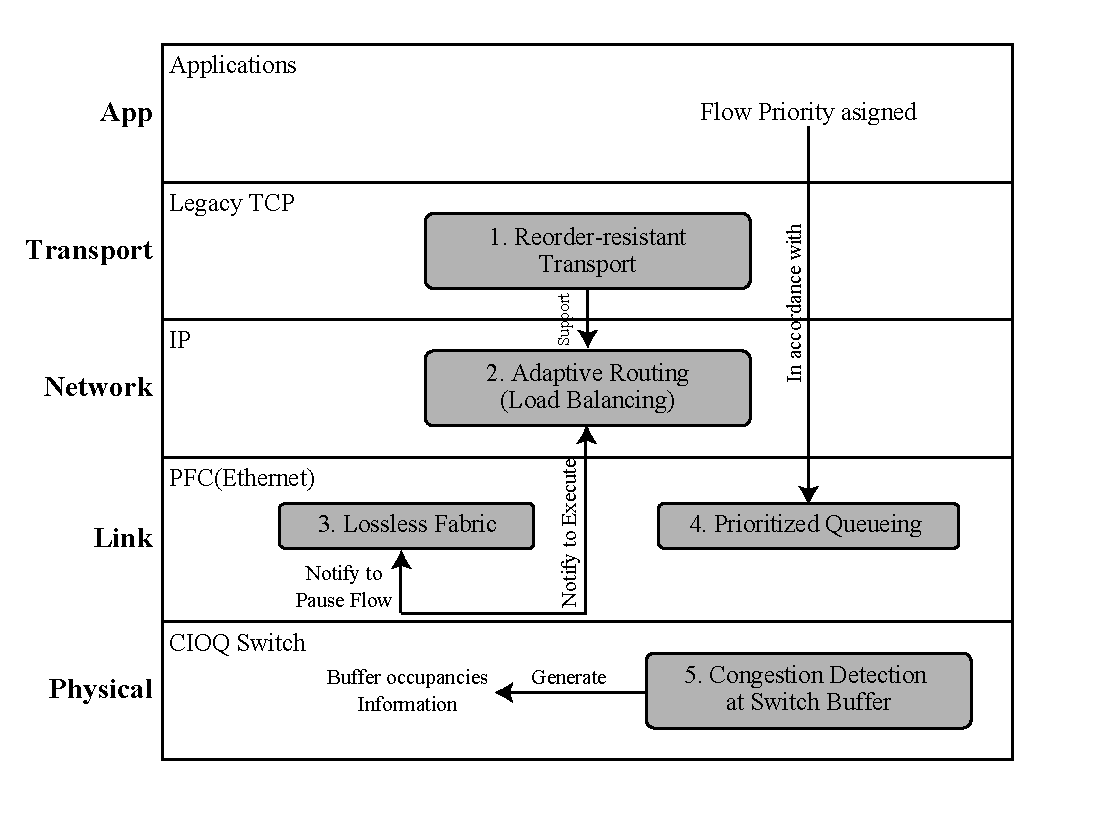
\includegraphics[autoebb, width=200pt]{./img/detal.pdf}
    \caption{DeTail's cross-layer design}
    %\ecaption{The control loop in DCTCP}
    \label{fig:detail_crosslayer}
    \end{center}
\end{figure}



\subsubsection{RepFlow}
これまでの遅延改善手法は, スイッチ, エンドノード, ネットワークスタック, あるいはネットワークファブリックそのものに対して変更が必要だった. 
RepFlow\cite{repflow}では, スイッチやエンドノードのカーネルに対する変更なしで,
ショートフローを複製し各経路に転送することでFCTの改善を目指す, 単純で効果的な手法である. 

RepFlowは, 例えばFatTreeトポロジー\cite{fattree}のような複数の経路が存在するネットワークでの経路の多様性に着目している.
バースト性のあるトラフィックによる一時的な輻輳状態やECMPによるハッシュの衝突は, 基本的には場所, 時間についてランダムに発生するものである. 
結果的に, 異なる経路における輻輳の度合いは統計上独立であると考えることができる. 
RepFlowでは, 複製されたフローと元のフローは高い確率で異なる経路を通り, その両方のフローがキューイング遅延が起こる可能性は小さい. 
Fig. \ref{fig:repflow_scheario}にホットスポットを回避できるシナリオを示す. 

データセンタートラフィックの特徴として,
90\%以上がショートフロー($\leq$100KB)で全体のデータ量のおよそ5\%のみの割合である\cite{dctcp,
p_fab}ことからショートフローの影響はとても小さいと考えることができる. 
さらに, RepFlowは他のトランスポートプロトコルとの互換性があり,
既存のTCPだけでなくDCTCP\cite{dctcp}に対しても適用することができる. 
Xuらはシミュレーション実験によってRepFlowの性能を評価し,
FCTの平均値と99パーセンタイル値の50\%$\sim$70改善することができたことを示した. 
\begin{figure}[t]
    \begin{center}
    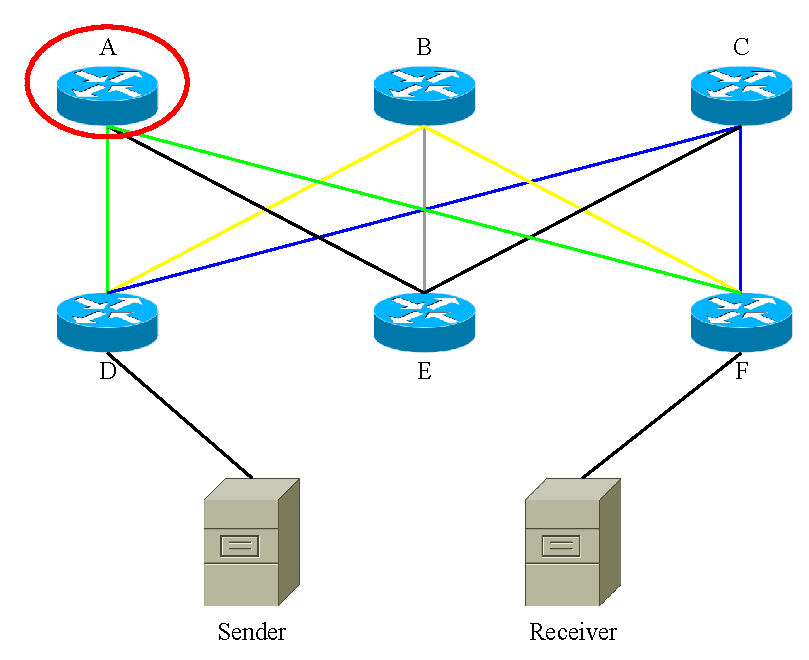
\includegraphics[autoebb, width=200pt]{./img/repflow_ie.pdf}
    \caption{An example to understand RepFlow}
    %\ecaption{The control loop in DCTCP}
    \label{fig:repflow_scheario}
    \end{center}
\end{figure}
% 
% \section{プロトコルに対するアプローチ}
% 2011年にCostinらによって, MPTCPを用いたデータセンターネットワークモデルが提案された~\cite{improving}.
% 近年の大規模計算資源を有効活用するために提案されたネットワークトポロジーでは,
% 高性能なデバイスや特殊な機器を必要とせず, 汎用的なネットワーク機器のみを用いてデータセンター内のエンドノード同士の通信に経路が複数用意されている.
% 既存の取り組みでは, 通信に使わない経路をセカンダリ経路として利用することで, 耐障害性を持たせていたのに対し, 提案されたデータセンターモデルでは,
% MPTCPを用い複数経路を同時に利用する事で, 耐障害性を保ちながら, 帯域を最大限利用する事を可能にした.
% また, 様々なトポロジーにMPTCPを適用することで, 従来のTCPよりも高いスループットが出せることを示した.
% しかし, MPTCPとSingle path-TCPが混在する環境において, Single
% path-TCPで行われるサイズの小さいフロー($\leq70KB$)のフロー完結時間に着目すると, 従来のSingle
% path-TCPのみのネットワーク環境よりも時間がかかるという問題点があった.
% 現状のMPTCPの実装では, サイズの小さいフローにおいてはサブフローを形成する前に通信が完了するので, MPTCPとSingle
% path-TCPが混在する環境は十分起こりうるものである\cite{mptcp_ana}.
% 
% 
% \section{スイッチに対するアプローチ}
% 2012年にZarsらによって, 複数レイヤー間でトラフィックを監視し,
% しきい値を設定することによるフロー完結時間の短縮化技術を提案した~\cite{detail}.
% 今日のデータセンター内ネットワークのような, サイズの異なるフローが混在するネットワークにおいては, サイズが小さいフローがサイズの大きいフローに圧迫され,
% 伝送遅延が大きくなる問題があったが, この提案手法では, データリンク層からアプリケーション層までの各層が,
% 相互にトラフィックを監視する機能をスイッチに実装し, 優先度をつけ, バッファサイズを調整することで, フロー完結時間の劣化を抑えることを可能にした.
% しかし, 実験ではClick~\cite{click}を用いて実装を行っており, 現実世界での全てのネットワーク機器の置き換えが必要となるので, 実現は難しい.
% 
% \section{アプリケーションに対するアプローチ}
% 2014年にH. Xuらによって, 通信可能な経路の数だけソケットを複製し, 通信環境が最も良い経路のフロー完結時間を採用することで,
% フロー完結時間を短縮化する技術を提案した\cite{repflow}.
% 今日のデータセンターでは, データセンター内のノード間の経路が複数存在し, それらに対して例えばECMPのようなハッシュベースの経路選択を行うと,
% 通信環境の悪い経路を選択する可能性がある.
% この提案手法では, スイッチやノードのOSに対しての変更を必要とせず, 極めて単純な仕組みによって, フロー完結時間の短縮化を実現している.
% しかし, 最もフロー完結時間が短かったもの以外のフローに対しては, ノード間の通信にとって無駄なものとなり, ネットワーク全体の通信量増加による,
% 新たな輻輳を発生させる.
% また, 比較的サイズの小さいフローのみこの手法は有効であり, サイズの大きいフローに対しては, 従来の通信をよりも時間がかかることが理論的に示されている.
% そのため提案手法では, 事前にフローサイズを把握しておき, 提案手法を適用するか否かを判断する必要があるため, アプリケーションに対して変更が必要となり,
% これを現実世界への適用を考えると, すべてのアプロケーションに対して変更が必要となり, 提案手法の実用化は困難であると言える.





\section{本研究の位置付け}
これまでの関連研究を踏まえて, キューイング遅延が生じている原因であるスイッチに対する変更により, 直接情報を取得し, 改善を行う傾向がある. 
しかし, 実環境への適用の点では, すべてのスイッチ機器の変更を加えることは現実的ではないと考える. 
近年のデータセンターネットワーク, またその上で稼働するアプリケーション性能向上の観点から, 以下のような要件が考えられる.
\begin{itemize}
  \item 大規模計算機を有効活用するトポロジーの利用
  \item 分散処理の際に発生する大量のサイズの小さいフローの送信時間の短縮
  \item 特殊な実装やデバイスを用いず, 汎用的でシームレスな運用の実現
\end{itemize}
本研究ではこれらの要求案件を満たす, データセンターでのショートフローの改善手法を提案する. 
